\chapter{The Search for $\boldmath{t+p_\text{T}^\text{miss}}$}

In this chapter, we discuss the search for dark matter produced in association with a single top quark (``mono-top'').
Since the initial state of $pp$ collisions do not contain any appreciable contribution from top quarks, any process that produces a single top quark must involve some flavor violation.
In the Standard Model, any such process is heavily suppressed by off-diagonal elements of the CKM matrix.
The SM production mechanism for the mono-top signature (Fig.~\ref{fig:tzq}) involves a $b$ quark in the final state, and thus does not couple the third generation with the first or second.
True production of mono-top must introduce some such coupling as an extension to the SM, in addition to one (or more) invisible particle to serve as a DM candidate.

\begin{figure}
    \begin{center}
        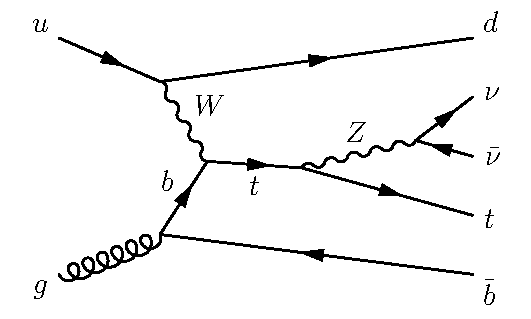
\includegraphics[width=0.5\textwidth]{figures/monotop/diagrams/tzq.pdf}
        \caption{Production of mono-top in the SM, in which a top quark is produced in addition to a $Z$ boson and bottom quark. The $Z$ decays to neutrinos, providing large \ptmiss.}
        \label{fig:tzq}
    \end{center}
\end{figure}

To illustrate how beyond-SM physics can produce this final state, we introduce two DM models: a flavor-changing neutral current $V$ and a charged, colored scalar $\phi$.
These models will also be used to benchmark the sensitivity of the analysis.
However, it should be emphasized that the search is motivitated and designed agnostically, without reliance on any specific model; the assumption is that the mono-top final state alone is indicative of new physics, regardless of the specific production mechanism.

The FCNC $V$ is assumed to couple to a fermionic DM candidate $\chi$. 
A partial Lagrangian of the interaction terms is given by:
\begin{equation}
\mathcal{L}_\text{int}=  V_\mu  \overline\chi \gamma^\mu (  g^V_{\chi} + g^A_{\chi} \gamma_5 ) \chi
                           + \overline{q}_u \gamma^\mu
                           ( g^V_u + g^A_u \gamma_5 ) q_u V_\mu
                           + \overline{q}_{d} \gamma^\mu
                           (  g^V_{d} + g^A_{d} \gamma_5 ) q_d V_\mu
                           + \text{h.c.},
    \label{eq:Lfcnc}
\end{equation}
The model comes with 22 free parameters, broadly organized in three sets:
\begin{itemize}
    \item The masses $m_V$ and $m_\chi$. (2)
    \item The couplings $g_\chi^V$ and $g_\chi^A$. These, respectively, control the strength of the vector and axial interactions between $V$ and $\chi$. (2)
    \item The four coupling matrices $g_{q}^{X}$, where $q=u,d$ and $X=V,A$. 
          As before, $X$ determines the type of spin-1 interaction. 
          In principle, different coupling strengths can be permitted for up- and down-type quarks, so this indexed by $q$. 
          Each $g_{q}^{X}$ is a $3\times3$ matrix, cross-coupling the three quark generations. 
          To preserve $\mathrm{SU}(2)_\mathrm{L}$ symmetry, we require $g_u^V - g_u^A = g_d^V - g_d^A$. ($3\times6=18$)
\end{itemize}

It is the $g_{u,d}^{V,A}$ that determines whether the model can produce mono-top, or mono-bottom, or mono-up, etc. 
If $g_{u,d}$ is strongly diagonal (i.e. strongest couplings are within generations), then mono-light quark production will dominate, resulting in the mono-jet final state (Fig~\ref{fig:fcncdiaga}).
On the other hand, if we assume the only non-zero elements are those that couple the first and third generations, then mono-top production at the LHC is the best way to probe this model (Fig~\ref{fig:fcncdiagb}).

\begin{figure}
    \begin{center}
        \begin{subfigure}[t]{0.49\textwidth}
            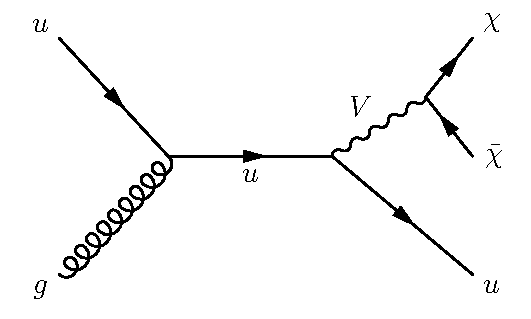
\includegraphics[width=\textwidth]{figures/monotop/diagrams/mj.pdf}
            \caption{mono-jet}
            \label{fig:fcncdiaga}
        \end{subfigure}
        \begin{subfigure}[t]{0.49\textwidth}
            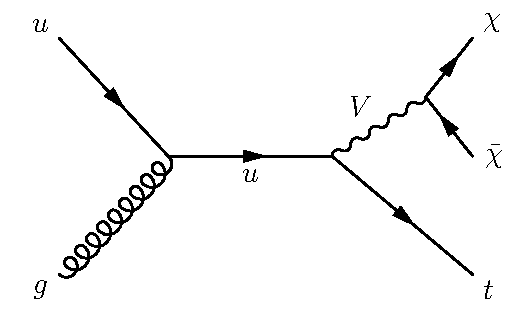
\includegraphics[width=\textwidth]{figures/monotop/diagrams/fcncb.pdf}
            \caption{mono-top}
            \label{fig:fcncdiagb}
        \end{subfigure}
        \caption{Possible DM production at the LHC, assuming a simplified spin-1 extension to the SM. Left: if the coupling matrix is dominated by diagonal elements, mono-jet production is enhanced. Right: if $(g_{u}^{V,A})_{ij} \approx \delta_{i1}\delta_{j3} + \delta_{i3}\delta_{j1}$, then mono-top production is dominant.}
        \label{fig:fcncdiag}
    \end{center}
\end{figure}
    

\section{Signal selection}

\section{Background estimation}

\subsection{Visible final states to constrain invisible final states}

\subsection{Theoretically-limited extrapolations}

\section{Results}

\subsection{Constraints on spin-1 FCNCs}

\subsection{Constraints on scalar resonances}

\subsection{Extending to new BSM models}
